% !TEX root = /doc.tex

\section{Evaluation}

\subsection{Evaluation metrics}

The evaluation metrics collected to compare the classifiers come from the field of information retrieval and are considered standard metrics for their purpose \cite{Sammut2017}. Most of these metrics can be calculated using values from a so-called confusion matrix and all of them measure the performance of the predictions of classifiers from different points of view. In the case of a binary classification, as this work was based on, this matrix consists of four groups whose values indicate whether the respective classifier could correctly or incorrectly assign an object to one of the two target classes \cite{Sammut2017}. In connection with such matrices, the two target classes are called "positive" and "negative". For this work the positive class is assigned to the label "defective" and the negative class to the label "clean". The form of a general confusion matrix is shown in \autoref{fig:confu}.

\begin{figure}[H]
    \centering
    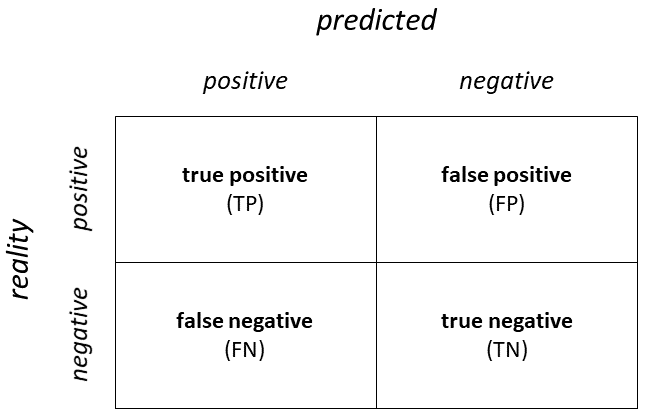
\includegraphics[width=0.4\textwidth]{Confusion}
    \caption{general confusion matrix\label{fig:confu}}
\end{figure}

The WEKA tool used for training the classifiers has the option of outputting confusion matrices for the tests performed on the classifiers. Based on the values of the assignments to the groups mentioned above, the following evaluation metrics were calculated:

\begin{itemize}
\item Accuracy
\\This value measures the accuracy of the classifier's predictions and indicates to what extent its predictions agree with the modelled reality \cite{Sammut2017}. The formula for calculating the accuracy is:
\\\[\text{Accuracy} = \frac{TP+TN}{TP+TN+FP+FN}\]
The result of the calculation is a percentage value. $100\%$ represents the best possible accuracy. In this case, all predictions are correct and correspond to reality.
\item True-Positive-Rate (TP rate) / Recall
\\This value indicates the proportion of correctly positive predictions of all positive predictions \cite{Alpaydin2010}. The formula for calculating the TP rate or recall is
\\\[\text{TP rate} = \frac{TP}{TP+FN}\]
The result of the calculation is a percentage value. $100\%$ thus represents the best possible TP rate or recall. In this case all positive predictions are made correctly. Both terms are used in parallel to calculate the formula shown.
\item Precision
\\ This value indicates the number of positive predictions that actually belong to the positive class \cite{Sammut2017}. The formula for determining the precision is
\\\[\text{Precision} = \frac{TP}{TP+FP}\]
The result of the calculation is a percentage value. $100\%$ represents the best possible precision. In this case only correct positive predictions are made.
\item F score
\\ This value calculates the harmonic mean of the Precision and Recall values and is therefore between these two values, but closer to the smaller value \cite{Sammut2017}. The formula for calculating the F score is
\\\[\text{F score} = \frac{2TP}{2TP+FP+FN}\]
The result of the calculation is a percentage value. $100\%$ represents the best possible F score. In this case, all positive predictions were made correctly.
\end{itemize}

In order to obtain a further measure of the prediction performance and the quality of the predictions, the so-called ROC curves (ROC = Receiver Operating characteristic) of the individual classifiers were determined. These have the advantage that they represent the performance of the classifiers in a simple and understandable way and make the quality of the predictions "visible". For this purpose, it is sufficient to know the standard progression of the curves, which will be illustrated in the following example.
The ROC curves are probability distributions that describe the relationship between the TP rate (y axis) and the false positive rate (x axis) \cite{Sammut2017}. The False-Positive-Rate (FP rate) indicates the proportion of predictions that are incorrectly evaluated as positive \cite{Alpaydin2010}. It is calculated using the following formula:
\\\[\text{FP rate} = \frac{FP}{FP+TN}\]
As with all metrics, the result of the FP rate is a percentage value. In contrast to the previous metrics, this result should at best be as low as possible. Both the TP rate and the FP rate give only singular values, from which no graphs can be derived. However, when predicting a data point, each classifier calculates probabilities that represent the affiliation to the values of the target class. As a rule, a data point is assigned to the positive class if the probability exceeds a threshold value of $0.5$ - data points that fall below this threshold value are assigned to the negative class. If the threshold value is increased, fewer data points are assigned to the positive class, whereas if the threshold value is lowered, more data points are assigned to the positive class. For the creation of the ROC curves, the values of the TP rate and FP rate are thus compared, taking into account the threshold values in the range of $0.0$ to $1.0$.

Another metric that occurs in conjunction with the ROC curve is the AUC area. This value, which is calculated using the ROC curve (AUC = area under curve), indicates the extent to which a classifier is able to distinguish between the values of the target classes. The higher this value is ($1.0$ is the maximum), the better the classifier can make correct predictions. It therefore reflects the quality of the predictions.
All presented metrics are automatically calculated by WEKA. The tool also has the ability to output ROC curves with the corresponding AUC areas. The values of the metrics determined during the evaluation of the classifiers as well as the ROC curves and AUC areas are listed, compared and interpreted in the following section.

\subsection{Results}

This chapter serves to evaluate the classifiers explained in the previous chapter, which are based on the three data sets presented and were built on the basis of data from 12 feature-based software projects. These are the feature-based dataset, the "simple" and the extended file-based dataset, which additionally contains the metrics of the feature-based dataset, mapped on file level. The data sets consist of the attributes and the label as columns and in the rows the corresponding values for each feature or file aggregated by release. The evaluation is done by different evaluation metrics and based on values of so-called confusion matrices and ROC curves. This part of the evaluation is extended with the comparison between the "simple" and extended file-based dataset to measure the influence of the feature-based metrics on the performance of the predictions.

\subsubsection*{Results and comparison of the feature-based classifiers}

The presentation of the results starts with those of the classifiers of the feature-based data set. Based on the results of the evaluation metrics, performance can be measured and interpreted in terms of predicting faulty or error-free features. 

\paragraph{Confusion matrices}
The confusion matrices serve as a basis for the results of the evaluation of the classifiers using the metrics presented above. The matrices of the feature-based dataset are listed in \autoref{tab:mat-feat}. The columns represent the labels predicted by the classifiers. The rows in turn represent the "ground truth", i.e. the reality determined during the creation of the datasets. Furthermore, the determined values of the respective classes are added together in the columns "total". Since the same test set was selected for each classifier, the values in the "total" column are identical. The abbreviations used for the classifiers can be found in \autoref{tab:classifiers}.

\begin{table}[t]
\centering
\caption{Confusion matrices of the feature-based data set}
\label{tab:mat-feat}
\begin{tabular}{@{}lllrr@{}}
\toprule
\multicolumn{1}{c}{} & predicted -\textgreater{} & defecive & clean   & total   \\ \midrule
\multirow{3}{*}{J48} & real defective            & $446$    & $320$   & $766$   \\
                     & real clean                & $483$    & $3.142$ & $3.625$ \\
                     & total                     & $929$    & $3.462$ & $4.391$ \\ \midrule
\multirow{3}{*}{KNN} & real defective            & $371$    & $395$   & $766$   \\
                     & real clean                & $569$    & $3.056$ & $3.625$ \\
                     & total                     & $940$    & $3.451$ & $4.391$ \\ \midrule
\multirow{3}{*}{LR}  & real defective            & $309$    & $457$   & $766$   \\
                     & real clean                & $1.020$  & $2.605$ & $3.625$ \\
                     & total                     & $1.329$  & $3.061$ & $4.391$ \\ \midrule
\multirow{3}{*}{NB}  & real defective            & $322$    & $444$   & $766$   \\
                     & real clean                & $265$    & $3.360$ & $3.625$ \\
                     & total                     & $587$    & $3.804$ & $4.391$ \\ \midrule
\multirow{3}{*}{NN}  & real defective            & $327$    & $439$   & $766$   \\
                     & real clean                & $1.019$  & $2.60$6 & $3.625$ \\
                     & total                     & $1.346$  & $3.045$ & $4.391$ \\ \midrule
\multirow{3}{*}{RF}  & real defective            & $504$    & $262$   & $766$   \\
                     & real clean                & $450$    & $3.175$ & $3.625$ \\
                     & total                     & $954$    & $3.437$ & $4.391$ \\ \midrule
\multirow{3}{*}{SGD} & real defective            & $251$    & $515$   & $766$   \\
                     & real clean                & $938$    & $2.687$ & $3.625$ \\
                     & total                     & $1.189$  & $3.202$ & $4.391$ \\ \midrule
\multirow{3}{*}{SVM} & real defective            & $176$    & $590$   & $766$   \\
                     & real clean                & $899$    & $2.726$ & $3.625$ \\
                     & total                     & $1.075$  & $3.316$ & $4.391$ \\ \bottomrule
\end{tabular}
\end{table}

\paragraph{Accuracy, TP rate / recall, FP rate, precision, F-score}

The results of these metrics are presented in \autoref{tab:met-results-feat}. The results show that the Accuracies of the classifiers are between $66\%$ and $84\%$. The classifiers NB and RF achieved the highest values with a hit accuracy of $84\%$ each. With a value of $82\%$, the J48 classifier also achieved above-average performance. This was followed by the KNN classifier with $78\%$. With values of $66\%$ and $67\%$ respectively, the classifiers LR, NN, SGD and SVM performed the worst. Thus, they determined a wrong result in more than $30\%$ of the predictions. What is striking about these results is the high performance of both decision tree-based classifiers J48 and RF. Thus, they seem to be best able to process the input quantity in order to draw conclusions about the new data in the form of test data.

The results of the further evaluation metrics TP rate / recall, FP rate, precision and F-score are divided according to the values of the target class, "defective" and "clean". In addition, the mean value of the results of both values of the target class is given. It displays the performance aggregated for both values and is ideally $1.00$ or $0.00$ for the FP rate.

A first look at the results of the evaluation metrics shows that the results (with the exception of the FP rate) related to the label "defective" are worse than those of the label "clean". The best results in comparison were achieved by the RF classifier for the label "defective". $66\%$ of the actually defective data points were also predicted as such and only $12\%$ of the data points were falsely predicted as defective. The Precision and F-Score values are $53\%$ and $59\%$ respectively, at an average level. The J48 classifier achieved comparable results. SGD and SVM have the worst overall values. They actually detected defective data points with an accuracy of $34\%$ and $23\%$ respectively. The other classifiers operated at an average level. The respective mean values can be considered to compare the overall performance of the classifiers for both labels. Here again, the RF classifier performs best. The values for TP rate, precision and F-score are in the range of over $73\%$ and are thus comparatively above average. The FP rate of $23\%$, which is mainly due to the results regarding the label "clean", is at the lowest level of all classifiers. Again, the results of the decision tree based classifier J48 are at a similar level. The classifiers KNN and NB show average performance due to their high FP rate values. In total, the values of the classifiers LR, NN, SGD and SVM show that they have the worst performance in comparison. Especially the FP rates of over $43\%$ are at a high, undesirable level. 


\begin{table}[t]
\centering
\caption{Results of the evaluation metrics of the feature-based data set}
\label{tab:met-results-feat}
\begin{tabular}{@{}llrrr@{}}
\toprule
                     &                  & defective      & clean      & mean   \\ \midrule
\multirow{5}{*}{J48} & accuracy         & \multicolumn{2}{r}{result:} & $0,82$ \\
                     & TP rate / recall & $0,58$         & $0,87$     & $0,73$ \\
                     & FP rate          & $0,13$         & $0,42$     & $0,28$ \\
                     & precision        & $0,48$         & $0,91$     & $0,70$ \\
                     & F-score          & $0,53$         & $0,89$     & $0,71$ \\ \midrule
\multirow{5}{*}{KNN} & accuracy         & \multicolumn{2}{r}{result:} & $0,78$ \\
                     & TP rate / recall & $0,48$         & $0,86$     & $0,67$ \\
                     & FP rate          & $0,16$         & $0,52$     & $0,68$ \\
                     & precision        & $0,40$         & $0,89$     & $0,65$ \\
                     & F-score          & $0,44$         & $0,86$     & $0,66$ \\ \midrule
\multirow{5}{*}{LR}  & accuracy         & \multicolumn{2}{r}{result:} & $0,66$ \\
                     & TP rate / recall & $0,40$         & $0,72$     & $0,56$ \\
                     & FP rate          & $0,28$         & $0,60$     & $0,44$ \\
                     & precision        & $0,23$         & $0,85$     & $0,54$ \\
                     & F-score          & $0,30$         & $0,78$     & $0,54$ \\ \midrule
\multirow{5}{*}{NB}  & accuracy         & \multicolumn{2}{r}{result:} & $0,84$ \\
                     & TP rate / recall & $0,42$         & $0,93$     & $0,68$ \\
                     & FP rate          & $0,07$         & $0,58$     & $0,33$ \\
                     & precision        & $0,55$         & $0,88$     & $0,72$ \\
                     & F-score          & $0,48$         & $0,91$     & $0,70$ \\ \midrule
\multirow{5}{*}{NN}  & accuracy         & \multicolumn{2}{r}{result:} & $0,67$ \\
                     & TP rate / recall & $0,43$         & $0,72$     & $0,58$ \\
                     & FP rate          & $0,28$         & $0,57$     & $0,43$ \\
                     & precision        & $0,24$         & $0,86$     & $0,55$ \\
                     & F-score          & $0,31$         & $0,78$     & $0,55$ \\ \midrule
\multirow{5}{*}{RF}  & accuracy         & \multicolumn{2}{r}{result:} & $0,84$ \\
                     & TP rate / recall & $0,66$         & $0,88$     & $0,77$ \\
                     & FP rate          & $0,12$         & $0,34$     & $0,23$ \\
                     & precision        & $0,53$         & $0,92$     & $0,73$ \\
                     & F-score          & $0,59$         & $0,90$     & $0,75$ \\ \midrule
\multirow{5}{*}{SGD} & accuracy         & \multicolumn{2}{r}{result:} & $0,67$ \\
                     & TP rate / recall & $0,34$         & $0,74$     & $0,54$ \\
                     & FP rate          & $0,56$         & $0,67$     & $0,62$ \\
                     & precision        & $0,21$         & $0,84$     & $0,53$ \\
                     & F-score          & $0,26$         & $0,79$     & $0,53$ \\ \midrule
\multirow{5}{*}{SVM} & accuracy         & \multicolumn{2}{r}{result:} & $0,66$ \\
                     & TP rate / recall & $0,23$         & $0,75$     & $0,48$ \\
                     & FP rate          & $0,25$         & $0,77$     & $0,51$ \\
                     & precision        & $0,16$         & $0,82$     & $0,49$ \\
                     & F-score          & $0,19$         & $0,79$     & $0,49$ \\ \bottomrule
\end{tabular}
\end{table}

\paragraph{ROC curves und AUC areas}

The interpretation of the ROC curves and ROC ranges is based on the presented scheme. The ROC curves are shown together with the values of the AUC ranges. The plots output by WEKA and unchanged are shown. The displayed colour gradients of the curves do not illustrate any information relevant for this purpose and can therefore be ignored.

\begin{figure*}[t]
  \centering
  \subfloat[][J48\\AUC = $0,77$]{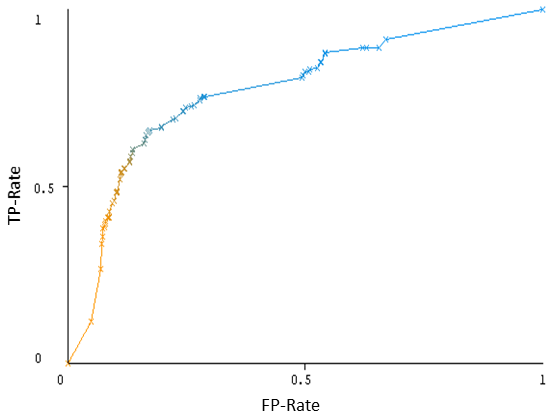
\includegraphics[width=0.25\linewidth]{j48_feat}} 
  \subfloat[][LR\\AUC = $0,62$]{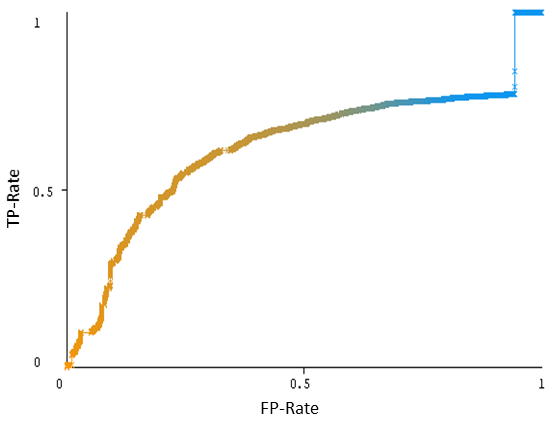
\includegraphics[width=0.25\linewidth]{lr_feat}}
  \subfloat[][NN\\AUC = $0,61$]{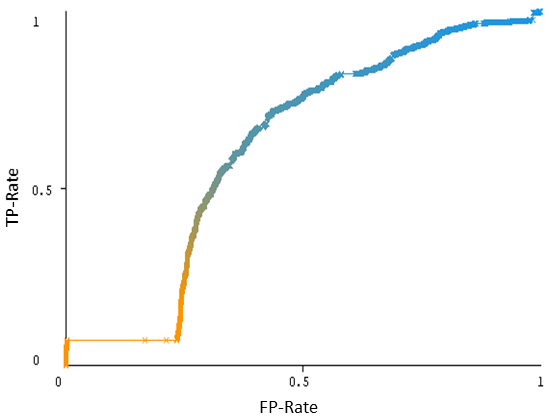
\includegraphics[width=0.25\linewidth]{nn_feat}}
  \subfloat[][SGD\\AUC = $0,53$]{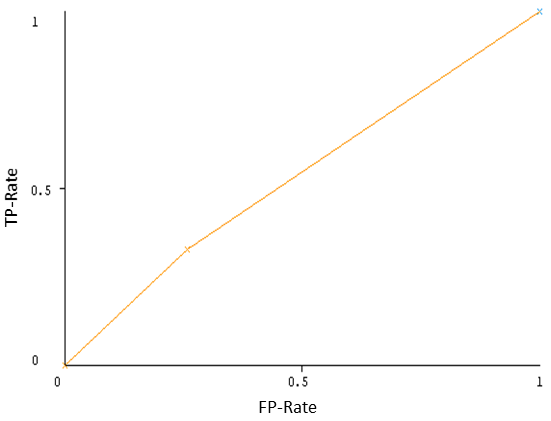
\includegraphics[width=0.25\linewidth]{sgd_feat}}
  \qquad
  \subfloat[][KNN\\AUC = $0,73$]{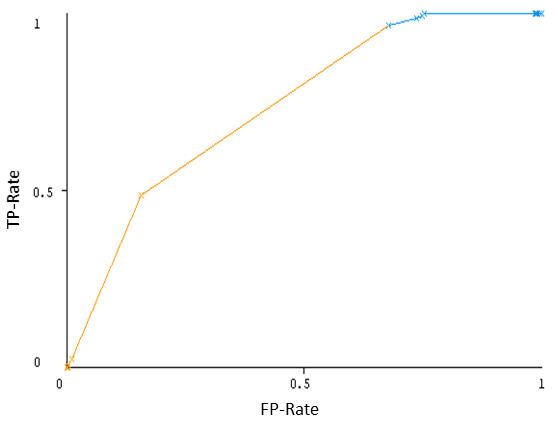
\includegraphics[width=0.25\linewidth]{knn_feat}}
  \subfloat[][NB\\AUC = $0,80$]{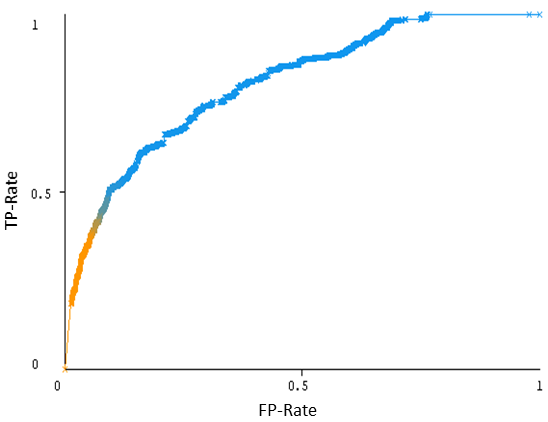
\includegraphics[width=0.25\linewidth]{nb_feat}}
  \subfloat[][RF\\AUC = $0,84$]{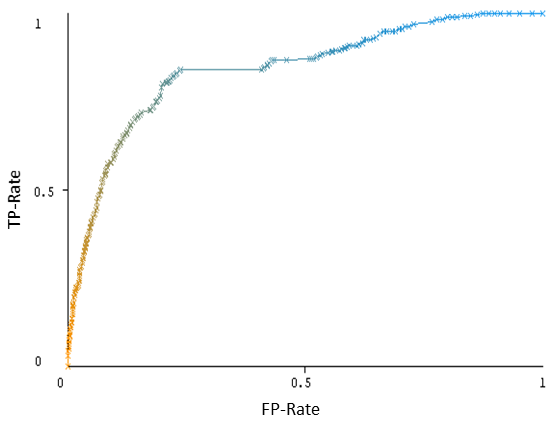
\includegraphics[width=0.25\linewidth]{rf_feat}} 
  \subfloat[][SVM\\AUC = $0,49$]{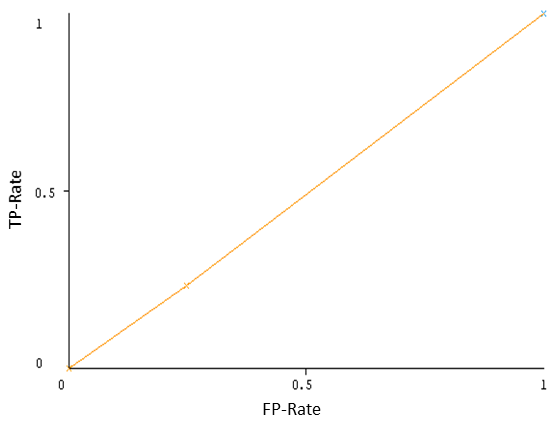
\includegraphics[width=0.25\linewidth]{svm_feat}}
  \caption{ROC curves of the feature-based data set \label{fig:roc-feat}}
\end{figure*}

It can be seen that no ROC curve approximates the ideal case presented. The best prediction performance is again shown by the RF Classifier with a AUC area of $0.84$. The NB Classifier shows a slightly lower performance with a ROC range of $0.80$. The classifiers J48 and KNN show an average performance of $0.77$ and $0.72$, respectively, with respect to the AUC area. The performance of the LR and NN classifiers are in the lower average. The SGD and SVM classifiers show the undesired case of a ROC curve bisecting the angle. This is also reflected in the AUC areas. The predictions thus approach a random guessing instead of being precise as desired.

\paragraph{Summary}

In each of the categories of metrics considered, the J48 and RF decision-tree-based classifiers proved to be the most performant compared to the other classifiers. The RF classifier usually also achieved a slightly higher performance. The algorithms underlying the classifiers seem to be best able to process the given feature-based data set with its eleven attributes with respect to the development of the derivation function for predicting new data.

The classifiers SGD and SVM always showed the worst performance in comparison for each category of evaluation metrics. It was also found that the predictions of these classifiers approached random rates. Thus, the feature-based dataset does not seem to be suitable for these classification algorithms. Reasons for this could be a too small number of instances or a too high number of attributes.

\subsubsection*{Results and comparison of the file-based classifiers}

This section is used to evaluate and compare the classifiers of the file-based data sets. The reason for this comparison is to measure the influence of the feature-based metrics on the predictions of a classical file-based method taken from the scientific literature \cite{Moser2008}. The division of this section is similar to the previous section. By considering the results of the evaluation metrics of both data sets, the influence of the feature-based metrics in the extended file-based data set on the performance of the predictions can be analyzed. 

\paragraph{Confusion matrices}

The confusion matrices of the file-based datasets are listed in \autoref{tab:mat-eval}. The parent columns are arranged into the "simple" and the extended dataset. Both datasets contain the same number of records, so the "total" columns are identical. A brief analysis of the "defective" - "real defective" fields shows that only very few actually defective data points were actually predicted to be defective. This is also reflected in the further results of the evaluation metrics.

\begin{table}[t]
\centering
\caption{Confusion matrices of the file-based data sets}
\label{tab:mat-eval}
\resizebox{\linewidth}{!}{%
\begin{tabular}{llrrrrrr} 
\toprule
                     &                & \multicolumn{3}{c}{„simple“ file-based data set} & \multicolumn{3}{c}{extended file-based data set}  \\ 
\midrule
\multicolumn{1}{c}{} & predicted -    & defective & clean     & total                    & defective & clean     & total                     \\
\multirow{3}{*}{J48} & real defective & $11$      & $102$     & $113$                    & $15$      & $98$      & $113$                     \\
                     & real clean     & $911$     & $20.923$  & $21.834$                 & $1.120$   & $20.714$  & $21.834$                  \\
                     & total          & $922$     & $21.025$  & $21.947$                 & $1.135$   & $2.0812$  & $21.947$                  \\ 
\midrule
\multirow{3}{*}{KNN} & real defective & $29$      & $84$      & $113$                    & $20$      & $93$      & $113$                     \\
                     & real clean     & $5.209$   & $16.625$  & $21.834$                 & $4.861$   & $16.973$  & $21.834$                  \\
                     & total          & $5.238$   & $16.709$  & $21.947$                 & $4.881$   & $17.066$  & $21.947$                  \\ 
\midrule
\multirow{3}{*}{LR}  & real defective & $36$      & $77$      & $113$                    & $32$      & $81$      & $113$                     \\
                     & real clean     & $2.520$   & $19.314$  & $21.834$                 & $2.578$   & $19.256$  & $21.834$                  \\
                     & total          & $2.556$   & $19.391$  & $21.947$                 & $2.610$   & $19.337$  & $21.947$                  \\ 
\midrule
\multirow{3}{*}{NB}  & real defective & $77$      & $36$      & $113$                    & $83$      & $30$      & $113$                     \\
                     & real clean     & $18.700$  & $3.134$   & $21.834$                 & $18.750$  & $3.084$   & $21.834$                  \\
                     & total          & $18.777$  & $3.170$   & $21.947$                 & $18.833$  & $3.114$   & $21.947$                  \\ 
\midrule
\multirow{3}{*}{NN}  & real defective & $6$       & $107$     & $113$                    & $1$       & $112$     & $113$                     \\
                     & real clean     & $4.341$   & $17.493$  & $21.834$                 & $141$     & $21.693$  & $21.834$                  \\
                     & total          & $4.347$   & $17.600$  & $21.947$                 & $142$     & $21.805$  & $21.947$                  \\ 
\midrule
\multirow{3}{*}{RF}  & real defective & $7$       & $106$     & $113$                    & $4$       & $109$     & $113$                     \\
                     & real clean     & $382$     & $21.452$  & $21.834$                 & $366$     & $21.468$  & $21.834$                  \\
                     & total          & $389$     & $21.558$  & $21.947$                 & $370$     & $21.577$  & $21.947$                  \\ 
\midrule
\multirow{3}{*}{SGD} & real defective & $22$      & $91$      & $113$                    & $20$      & $93$      & $113$                     \\
                     & real clean     & $1.260$   & $20.574$  & $21.834$                 & $1.226$   & $20.608$  & $21.834$                  \\
                     & total          & $1.282$   & $20.665$  & $21.947$                 & $1.246$   & $20.701$  & $21.947$                  \\ 
\midrule
\multirow{3}{*}{SVM} & real defective & $22$      & $91$      & $113$                    & $21$      & $92$      & $113$                     \\
                     & real clean     & $1.041$   & $20.793$  & $21.834$                 & $991$     & $20.843$  & $21.834$                  \\
                     & total          & $1.063$   & $20.884$  & $21.947$                 & $1.012$   & $20.935$  & $21.947$                  \\
\bottomrule
\end{tabular}
}
\end{table}

\paragraph{Accuracy, TP rate / recall, FP rate, precision, F-score}

The results of these metrics are presented in \autoref{tab:met-results}. The parent columns are again represented by the two data sets.

\begin{table}[t]
\centering
\caption{Results of the evaluation metrics of the file-based data sets (TPR = TP rate)}
\label{tab:met-results}
\resizebox{\linewidth}{!}{%
\begin{tabular}{llrrrrrr} 
\toprule
                     &              & \multicolumn{3}{c}{"imple" file-based data set} & \multicolumn{3}{c}{extended file-based data set}  \\ 
\cline{3-8}
                     &              & defective & clean           & mean              & defective & clean           & mean                \\ 
\midrule
\multirow{5}{*}{J48} & accuracy     & \multicolumn{2}{r}{result:} & $0,95$            & \multicolumn{2}{r}{result:} & $0,94$              \\
                     & TPR / recall & $0,10$    & $0,96$          & $0,53$            & $0,13$    & $0,95$          & $0,54$              \\
                     & FP rate      & $0,04$    & $0,90$          & $0,47$            & $0,05$    & $0,87$          & $0,46$              \\
                     & precision    & $0,01$    & $1,00$          & $0,51$            & $0,01$    & $1,00$          & $0,51$              \\
                     & F-score      & $0,02$    & $0,98$          & $0,50$            & $0,02$    & $0,97$          & $0,50$              \\ 
\midrule
\multirow{5}{*}{KNN} & accuracy     & \multicolumn{2}{r}{result:} & $0,76$            & \multicolumn{2}{r}{result:} & $0,77$              \\
                     & TPR / recall & $0,26$    & $0,76$          & $0,51$            & $0,18$    & $0,78$          & $0,48$              \\
                     & FP rate      & $0,24$    & $0,74$          & $0,49$            & $0,22$    & $0,82$          & $0,47$              \\
                     & precision    & $0,01$    & $1,00$          & $0,51$            & $0,00$    & $1,00$          & $0,50$              \\
                     & F-score      & $0,01$    & $0,86$          & $0,44$            & $0,01$    & $0,87$          & $0,44$              \\ 
\midrule
\multirow{5}{*}{LR}  & accuracy     & \multicolumn{2}{r}{result:} & $0,88$            & \multicolumn{2}{r}{result:} & $0,89$              \\
                     & TPR / recall & $0,32$    & $0,89$          & $0,61$            & $0,28$    & $0,88$          & $0,58$              \\
                     & FP rate      & $0,12$    & $0,68$          & $0,40$            & $0,12$    & $0,72$          & $0,42$              \\
                     & precision    & $0,01$    & $1,00$          & $0,51$            & $0,01$    & $1,00$          & $0,51$              \\
                     & F-score      & $0,03$    & $0,94$          & $0,49$            & $0,02$    & $0,94$          & $0,48$              \\ 
\midrule
\multirow{5}{*}{NB}  & accuracy     & \multicolumn{2}{r}{result:} & $0,15$            & \multicolumn{2}{r}{result:} & $0,14$              \\
                     & TPR / recall & $0,68$    & $0,14$          & $0,41$            & $0,74$    & $0,14$          & $0,44$              \\
                     & FP rate      & $0,86$    & $0,32$          & $0,59$            & $0,86$    & $0,27$          & $0,57$              \\
                     & precision    & $0,00$    & $0,99$          & $0,50$            & $0,00$    & $0,99$          & $0,50$              \\
                     & F-score      & $0,01$    & $0,25$          & $0,13$            & $0,01$    & $0,25$          & $0,13$              \\ 
\midrule
\multirow{5}{*}{NN}  & accuracy     & \multicolumn{2}{r}{result:} & $0,80$            & \multicolumn{2}{r}{result:} & $0,99$              \\
                     & TPR / recall & $0,05$    & $0,80$          & $0,43$            & $0,01$    & $0,99$          & $0,50$              \\
                     & FP rate      & $0,20$    & $0,95$          & $0,58$            & $0,01$    & $0,99$          & $0,50$              \\
                     & precision    & $0,00$    & $0,99$          & $0,50$            & $0,01$    & $1,00$          & $0,51$              \\
                     & F-score      & $0,00$    & $0,89$          & $0,45$            & $0,01$    & $0,99$          & $0,50$              \\ 
\midrule
\multirow{5}{*}{RF}  & accuracy     & \multicolumn{2}{r}{result:} & $0,98$            & \multicolumn{2}{r}{result:} & $0,98$              \\
                     & TPR / recall & $0,06$    & $0,98$          & $0,52$            & $0,04$    & $0,98$          & $0,51$              \\
                     & FP rate      & $0,02$    & $0,94$          & $0,48$            & $0,02$    & $0,97$          & $0,50$              \\
                     & precision    & $0,02$    & $1,00$          & $0,51$            & $0,01$    & $1,00$          & $0,51$              \\
                     & F-score      & $0,03$    & $0,90$          & $0,47$            & $0,02$    & $0,99$          & $0,51$              \\ 
\midrule
\multirow{5}{*}{SGD} & accuracy     & \multicolumn{2}{r}{result:} & $0,94$            & \multicolumn{2}{r}{result:} & $0,94$              \\
                     & TPR / recall & $0,20$    & $0,94$          & $0,57$            & $0,18$    & $0,94$          & $0,56$              \\
                     & FP rate      & $0,06$    & $0,81$          & $0,44$            & $0,06$    & $0,82$          & $0,44$              \\
                     & precision    & $0,02$    & $1,00$          & $0,51$            & $0,02$    & $1,00$          & $0,51$              \\
                     & F-score      & $0,03$    & $0,97$          & $0,50$            & $0,03$    & $0,97$          & $0,50$              \\ 
\midrule
\multirow{5}{*}{SVM} & accuracy     & \multicolumn{2}{r}{result:} & $0,95$            & \multicolumn{2}{r}{result:} & $0,95$              \\
                     & TPR / recall & $0,20$    & $0,95$          & $0,58$            & $0,19$    & $1,00$          & $0,60$              \\
                     & FP rate      & $0,05$    & $0,81$          & $0,43$            & $0,05$    & $0,81$          & $0,43$              \\
                     & precision    & $0,02$    & $1,00$          & $0,51$            & $0,02$    & $1,00$          & $0,51$              \\
                     & F-score      & $0,04$    & $0,97$          & $0,51$            & $0,04$    & $0,98$          & $0,51$              \\
\bottomrule
\end{tabular}
}
\end{table}

The comparison between the accuracies of the data sets shows that the integration of feature-based metrics has no significant impact on the performance of the predictions for six out of eight classifiers. The achieved values of the Accuracies are on the same level there. The NB classifier achieves the worst accuracy in comparison with the other classifiers with about $15\%$ accuracy. It seems to be unable to process the high number of data sets correctly. The classifiers KNN and LR achieved above average results with about $76\%$ and $87\%$ respectively. With values of more than $90\%$, the classifiers J48, RF, SGD and SVM have extremely high values, whose validity should be questioned first. A consideration of the other evaluation metrics should be made.

The NN classifier shows a conspicuous behaviour. There is a clear jump in values of about $18\%$ between the "simple" and the extended data set. This anomaly should also be analyzed and interpreted using the other evaluation metrics. It may indicate that the classifier of the extended dataset can make more accurate predictions by adding the additional attributes, or that the predictions are negatively affected by the addition of the additional attributes, thus distorting the results.

The results of the further evaluation metrics of both data sets again show the trend that only a few defective data points were actually predicted as defective. With TP rates of $68\%$ and $74\%$ respectively, the NL classifiers achieved the highest hit rates. The other classifiers are significantly lower with values of $32\%$ at most. The other metrics of the "defective" columns also represent extremely weak results. Noticeable are the very high FP rates of the NB classifiers, which clearly weaken the good results of the TP rates.

The values of the "error-free" columns show very good values. Only the respective FP rates with over $68\%$ are clearly too high and show that the classifiers incorrectly predict many data points as "clean". An exception to this is again the NB classifiers, which achieved good values in terms of FP rates and precision, but have shortcomings in terms of TP rates and consequently the F-score. Furthermore, the different accuracies of the NN classifiers can be justified with the results of the other evaluation metrics. It can be seen that between the data sets the values of the TP rates and FP rates differ for both labels. Consequently, the F-scores also differ. These differences in the values lead to the different values of the Accuracies.

The mean values show that the overall results are strongly influenced downwards by the values of the "defective" columns. They show that all classifiers make predictions at an average to below average level.

\paragraph{ROC curves und AUC areas}

The ROC curves and their associated AUC areas of the file-based datasets can be seen in \autoref{roc-file}. Again, the displayed color gradients of the curves do not convey any information relevant for this purpose and can therefore be ignored.

A first look at the ROC curves of the classifiers shows a relatively uniform picture of curves that are very much oriented on the bisector and are uniform between the data sets. With the exception of the RF classifiers of both data sets, the curves with their associated ROC areas show a below-average to undesired performance (random rate of labels). With an ROC area of $0.71$, the RF classifiers have above average performance in the higher-level comparison.

The comparison between the NN classifiers shows that the classifier of the simple dataset shows the undesired behaviour and at the same time makes inverse predictions. This means that in some cases it predicts the label "defective" instead of "clean" and vice versa. The curve as well as the ROC area of the classifier of the extended dataset, however, only show the undesired behavior in the form of random guessing of the predictions. This shows that the high accuracies of the NN classifiers shown in \autoref{tab:met-results} are probably caused by chance. In a further application of the test data, the results could have been different.

\begin{figure*}[t]
  \centering
  \subfloat[][J48 "simple"\\AUC = $0,61$]{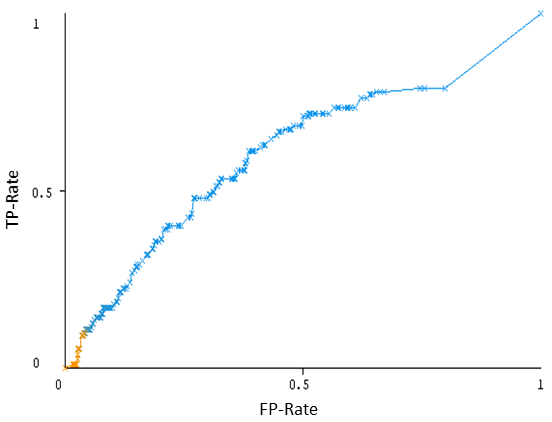
\includegraphics[width=0.25\linewidth]{j48_eval}} 
  \subfloat[][J48 extended\\AUC = $0,61$]{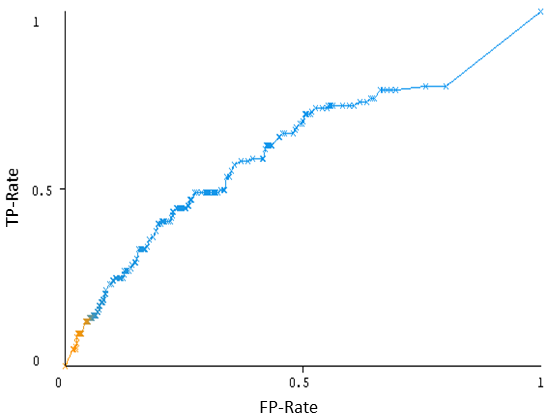
\includegraphics[width=0.25\linewidth]{j48_eval_feat}}
  \subfloat[][NN "simple"\\AUC = $0,37$]{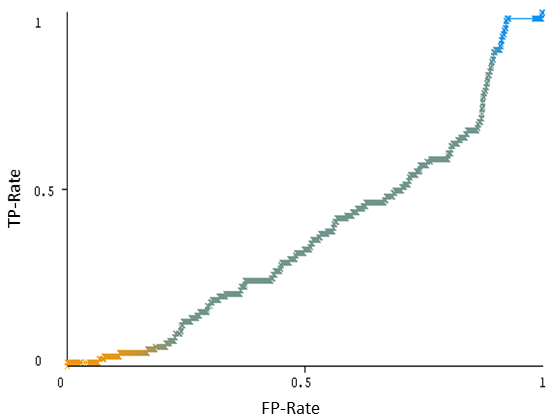
\includegraphics[width=0.25\linewidth]{nn_eval}}
  \subfloat[][NN extended\\AUC = $0,54$]{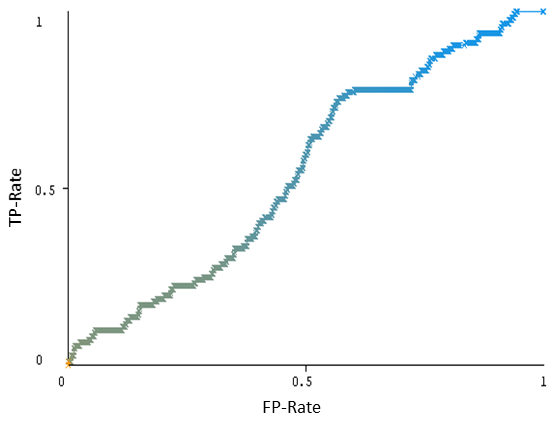
\includegraphics[width=0.25\linewidth]{nn_eval_feat}}
  \qquad
  \subfloat[][KNN "simple"\\AUC = $0,55$]{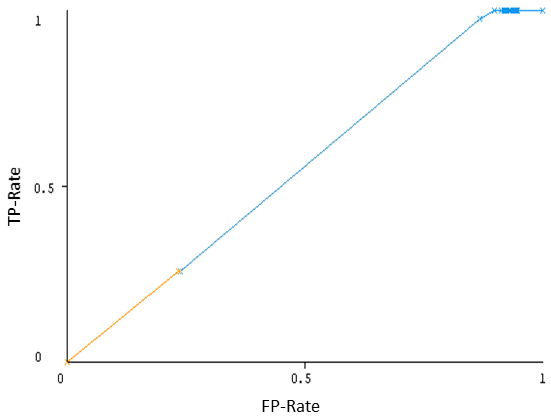
\includegraphics[width=0.25\linewidth]{knn_eval}}
  \subfloat[][KNN extended\\AUC = $0,52$]{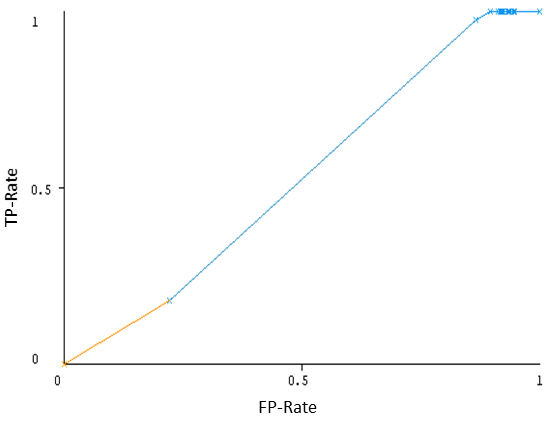
\includegraphics[width=0.25\linewidth]{knn_eval_feat}}
  \subfloat[][RF "simple"\\AUC = $0,71$]{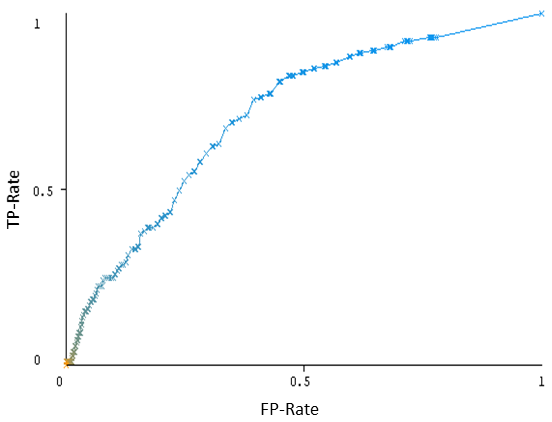
\includegraphics[width=0.25\linewidth]{rf_eval}} 
  \subfloat[][RF extended\\AUC = $0,71$]{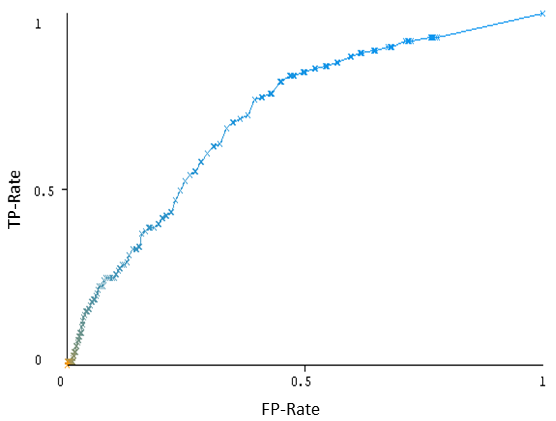
\includegraphics[width=0.25\linewidth]{rf_eval_feat}} 
  \qquad
  \subfloat[][LR "simple"\\AUC = $0,65$]{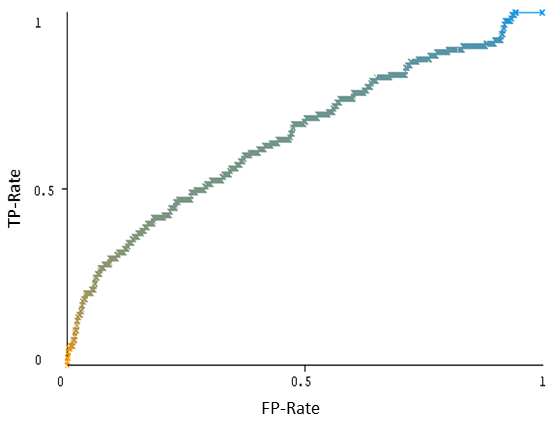
\includegraphics[width=0.25\linewidth]{lr_eval}}
  \subfloat[][LR extended\\AUC = $0,62$]{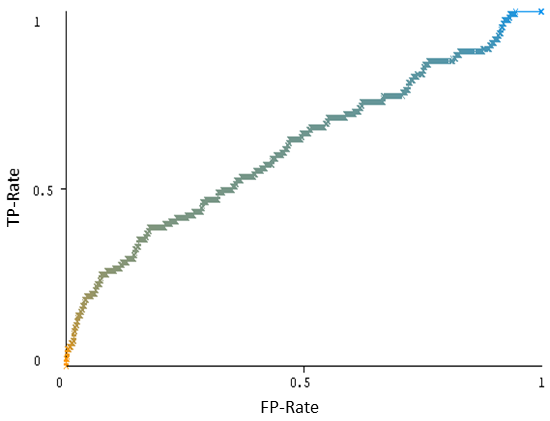
\includegraphics[width=0.25\linewidth]{lr_eval_feat}}
  \subfloat[][SGD "simple"\\AUC = $0,57$]{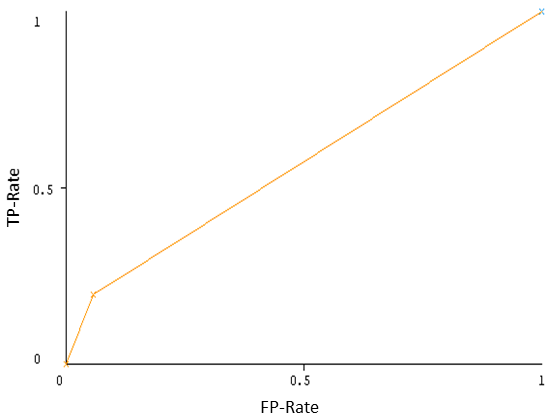
\includegraphics[width=0.25\linewidth]{sgd_eval}}
  \subfloat[][SGD extended\\AUC = $0,56$]{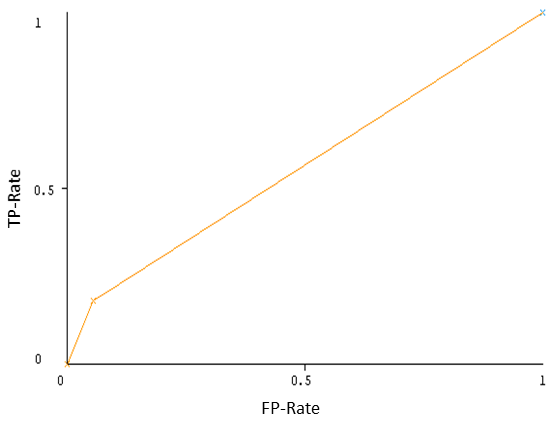
\includegraphics[width=0.25\linewidth]{sgd_eval_feat}}
  \qquad
  \subfloat[][NB "simple"\\AUC = $0,48$]{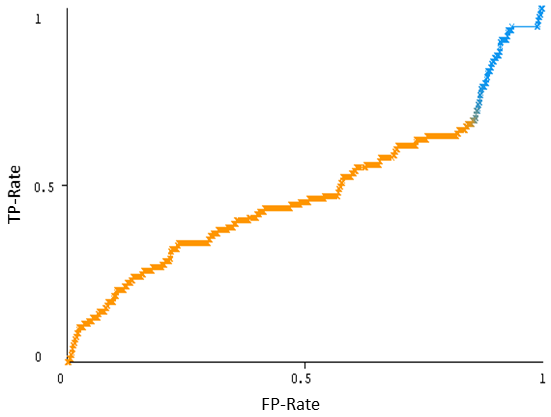
\includegraphics[width=0.25\linewidth]{nb_eval}}
  \subfloat[][NB extended\\AUC = $0,47$]{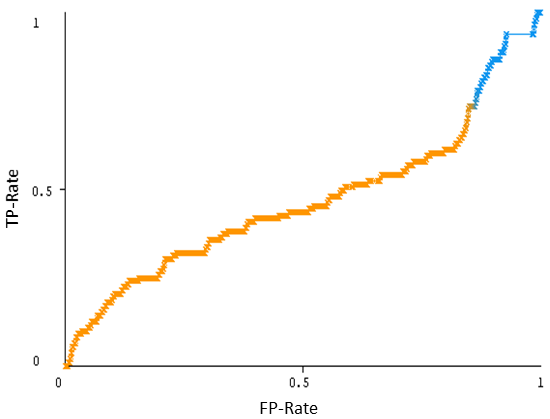
\includegraphics[width=0.25\linewidth]{nb_eval_feat}}
  \subfloat[][SVM "simple"\\AUC = $0,57$]{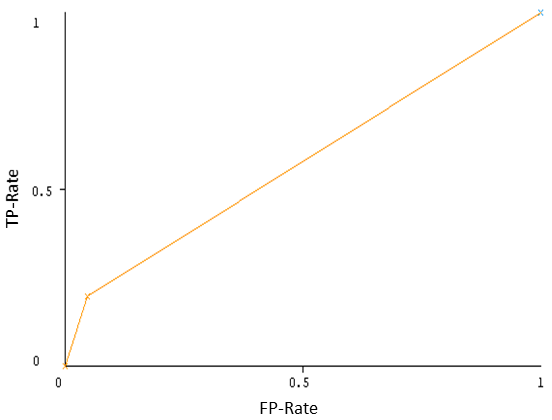
\includegraphics[width=0.25\linewidth]{svm_eval}}
  \subfloat[][SVM extended\\AUC = $0,57$]{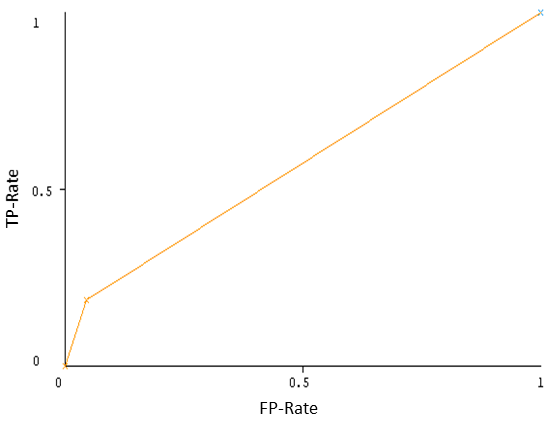
\includegraphics[width=0.25\linewidth]{svm_eval_feat}}
  \caption{ROC curves of the file-based data sets \label{roc-file}}
\end{figure*}

\paragraph{Summary}

The results of all metrics showed an undifferentiated and unclear picture of the classifier performance for both data sets. The reason for the shown results is the unbalanced nature of the respective test data sets with only $1\%$ of "defective" instances. In order to get good results for this label, many correct predictions have to be made by the classifiers. However, this was not the case for the existing test dataset, so that many predictions were incorrectly assigned to the dominant label "clean", which then, however, show high FP rates as a result. This is also reflected in the mean values in \autoref{tab:met-results}. Due to the significantly weaker values of the "defective" columns, the total values represented by the mean value are influenced downwards. However, as explained earlier, it is not intended to compensate for the unbalanced nature of the test data sets using the SMOTE algorithm.